\chapter{Markov Chain Monte Carlo}
\section{Gibbs Sampling}
% \label{sec:}

The phrase ``Markov chain Monte Carlo'' encompasses a broad array of techniques that have in common a few key ideas. The setup for all the techniques that we will discuss in this book is as follows:

\begin{enumerate}
	\item We want to sample from a some complicated density or probability mass function $\pi$. Often, this density is the result of a Bayesian computation so it can be interpreted as a posterior density. The presumption here is that we can evaluate $\pi$ but we cannot sample from it.
	\item We know that certain stochastic processes called Markov chains will converge to a stationary distribution (if it exists and if specific conditions are satisfied). Simulating from such a Markov chain for a long enough time will eventually give us a sample from the chain’s stationary distribution.
	\item Given the functional form of the density $\pi$, we want to construct a Markov chain that has $\pi$ as its stationary distribution.
	\item We want to sample values from the Markov chain such that the sequence of values $\{x_n\}$ generated by the chain converges in distribution to the density $\pi$.
\end{enumerate}

In order for all these ideas to make sense, we need to first go through some background on Markov chains. The rest of this chapter will be spent defining all these terms, the conditions under which they make sense, and giving examples of how they can be implemented in practice.

\section{Markov Chain}
\href{https://gregorygundersen.com/blog/2019/10/28/ergodic-markov-chains/}{Reference Link}

A Markov chain is a stochastic process that evolves over time by transitioning into different states. The sequence of states is denoted by the collection $\{X_i\}$ and the transition between states is random. Formally,
\begin{definition}
Let $D$ be a finite set. A random process $X_1, X_2,\dots$ with values in $D$ is called a Markov chain if
$$P(X_t=x_{t+1}|X_{t}=x_t,\dots,X_0=x_0)=P(X_{t+1}=x_{t+1}|X_{t}=x_t)$$
\end{definition}
We can think of $X_t$ as a random state at time $t$, and the Markovian assumption is that the probability of transitioning from $x_t$ to $x_{t+1}$ only depends on $x_t$. In other words, the future state depends only on the present. Let $p_{ij}$ be the probability of transitioning from state $i$ to state $j$. A Markov chain can be defined by a transition probability matrix:
\begin{definition}
	The matrix $\mathbf{P}=(p_{ij})_{i,j}\in D$ is called the transition probability matrix.
\end{definition}
Thus, $P$ is a $D \times D$ matrix, where $|D|$ denotes the cardinality of $D$, and the cell value $p_{ij}$ is the probability of transitioning from state $i$ to state $j$, and the rows of $P$ must sum to one. We will restrict ourselves to time \textit{homogeneous Markov chains}:

\begin{definition}
A Markov chain is called time homogeneous if 
$$\mathbb{P}\{X_{t+1}=j\, |\, X_n=i\}=p_{ij},\, \forall n.$$
\end{definition}
It state that \textit{the transition probabilities are not changing as a function of time}. Finally, let's introduce some useful notation for the initial state of the Markov chain. Let

$$\mathbb{P}_{x_0}\{\cdot\}\triangleq \mathbb{P}\{\cdot | X_0=x_0\}.$$

For example, I will write $\mathbb{P}_a\{X_1=b\}$ rather than $\mathbb{P}\{X_1=b|X_0=a\}$ for simplicity. 

Consider a simple Markov chain modeling the weather. The weather has two states: rainy and sunny. Thus, $D = \{r, s\}$ and $X_n$ is the ``weather on day $n$''. The Markov chain model is as follows. If today is rainy ($r$), tomorrow it is sunny ($s$) with probability $p$. If today it is sunny, tomorrow it is rainy with probability $q$. Then, transition matrix is given by 
\begin{align*}
	\mathbf{P} = 
	\begin{bmatrix}
		1-p & p\\
		q & 1-q
	\end{bmatrix}.
\end{align*}

The state diagram of the chain can be represented as follows:
\begin{figure}[h]
	\centering
	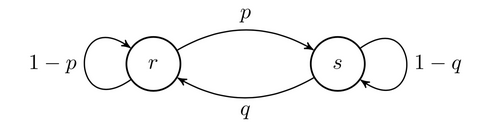
\includegraphics[scale=0.6]{./images/mcmc/transition_diagram.png}
	\caption{A sample Markov chain.}
	\label{fig:markov_chain_1}
\end{figure}
As a consequence of the Markovian assumptions, the probability of any path on a Markov chain is just the multiplication of the numbers along the path. For example, for some Markov chain with states $D=\{a, b, c, d\}$, the probability of a particular path, say $a\to b\to b\to d\to c$ factorize as 
$$p_{ab}\dots p_{dc}$$
Let's try to formulate this by
$$\mathbb{P}_i\{X_n=j\}.$$
For instance, let's say $n=2$. Then, we have
\begin{align*}
	\mathbb{P}_i\{X_2=j\} &= \sum_{d\in D}\mathbb{P}_i\{X_2=j, X_1=d\}\\
	&= \sum_{d\in D}\mathbb{P}_i\{X_2=j | X_1=d\}\mathbb{P}_i\{X_1=d\}\\
	&= \sum_{d\in D}p_{id}p_{dj}
\end{align*}
This is equivalent to a dot product of the $i$-th row to $j$-th column of the transition matrix $\mathbb{P}$. This can be expressed as follows:
$$\mathbb{P}\{X_2=j | X_0=i\} = \sum_{d\in D}p_{id}p_{dj} = \big(\mathbf{P}^2_{ij}\big).$$
This can be generalized to
$$\mathbb{P}_i\{X_n=j\} = \big(\mathbf{P}^n_{ij}\big).$$

\begin{figure}[h]
	\centering
	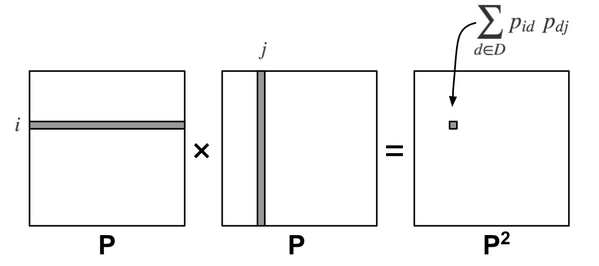
\includegraphics[scale=0.7]{./images/mcmc/transition_dot_product.png}
\end{figure}
In sum, the dot product performs marginalization, and everything works out nicely thanks to the Markovian assumption. If the $D$-dimensional vector $v$ represents a discrete distribution over initial states $X_0$, then $\bf v^T \bf P$ is a $D$-dimensional vector representing the probability distribution over $X_1$. 

\subsection{Ergodicity}

Let's discuss about \textit{ergodicity}, which is a property of a random process in which its time average is the same as its probability space average. It can be defined as follows:

\begin{definition}
A Markov chain $\{X_n\}$ is called ergodic if the limit
$$\boldsymbol{\pi} (j) = \lim_{n\to \infty}\mathbb{P}_i\{X_n=j\}$$
exists for every state $j$ and does not depend on the initial state $i$. The $D$-dimensional vector $\boldsymbol{\pi}(j)$ is called the stationary probability. 
\end{definition}
In other words, 
\begin{itemize}
	\item The probability $\boldsymbol{\pi}(j)$ of reaching at state $j$ (\ie $\mathbb{P}_i\{X_n=j\}$) 
	\item After a long time (\ie $\lim_{n\to\infty}$) 
	\item Regardless of the initial state $i$ (\ie $\mathbb{P}_i\{X_n=j\}$).
\end{itemize}
 Equivalently, it can be expressed as 
$$\boldsymbol{\pi}(j) = \lim_{n\to \infty}\big(\mathbf{P}^n\big)_{ij}.$$
The ergodicity gives the following property:
\begin{align*}
	\boldsymbol{\pi}(j) &= \lim_{n\to \infty}\big(\mathbf{P}^n\big)_{ij}\\ 
						&\overset{\star}{=} \lim_{n\to \infty}\big(\mathbf{P}^{n+1}\big)_{ij} \\
						&= \lim_{n\to \infty}\big(\mathbf{P}^{n}\mathbf{P}\big)_{ij} \\
						&= \lim_{n\to \infty}\sum_{d\in D}\big(\mathbf{P}^{n}\big)_{id}\mathbf{P}_{dj} \\
						&= \sum_{d\in D}\boldsymbol{\pi}(d)\mathbf{P}_{dj} \\
\end{align*}
\begin{itemize}
	\item The step $\star$ holds since the step $n$ and $n+1$ does not matter under the limit. 
\end{itemize}
Finally, we can write this as
$$\boldsymbol{\pi}^T = \boldsymbol{\pi}^T\mathbf{P},$$
where $\boldsymbol{\pi}$ is a column vector. Hence, the name ``stationary probability distribution'' denotes that it is a distribution that does not change over time. Note that it can be also written as:
$$\mathbf{P}^T\boldsymbol{\pi} = \boldsymbol{\pi}.$$
Then, we can say $\boldsymbol{\pi}$ is an eigenvector of $\mathbf{P}^T$ with eigenvalue of 1. Thus, we can obtain the stationary distribution $\boldsymbol{\pi}$ from an eigenvectors and eigenvalues of $\mathbf{P}^T$.


Since we are interested in ergodicity, let's now introduce some properties related to reachability and long-term behavior.

\begin{definition}
We say that there is a path from $i$ to $j$ ($i\rightsquigarrow j$) if there is a nonzero probability that starting at $i$, we can reach $j$ at some point in the future. 
\end{definition}

\begin{definition}
	A state $i$ is called \textbf{transient} if there exists a state $j$ such that $i\rightsquigarrow j$ but $j\not\rightsquigarrow i$.
\end{definition}

\begin{definition}
	A state $i$ is called \textbf{recurrent} if for all states $j$ there exist $i\rightsquigarrow j$ and $j\rightsquigarrow i$.
\end{definition}

\begin{definition}
A Markov chain is \textbf{\textit{irreducible}} if $i\leftrightarrow j, \forall i,j\in S$. Simply, if all states are able to visit other states, it is irreducible. 
\end{definition}

\begin{definition}
	State $i$ has a \textbf{period} $d$ (\ie periodically visit the state $i$) $\leftrightarrow$ aperiodic.
\end{definition}

Intuitively, a \textit{transient} state is a state that cannot return to itself; while a \textit{recurrent} state can return. In other words, these two conditions are opposite. A transient state is not recurrent, and a recurrent state is not transient. Note that if a state is recurrent, every reachable state is also recurrent. We think of a set of recurrent states as a "class" or a "recurrent class".
\begin{figure}[h]
	\centering
	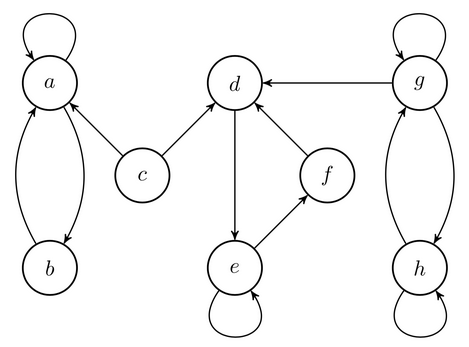
\includegraphics[scale=0.7]{./images/mcmc/markov_chain.png}
	\caption{A Markov chain with $D = \{a, b, c, d, e, f, g, h\}$. The state $c$ is a transient state. Note that $g$ and $h$ are also transient as there exist states that they cannot return. There are two recurrent classes: $\{a, b\}$ and $\{d, e, f\}$.}
	\label{fig:markov_chain_2}
\end{figure}
We can notice that \Cref{fig:markov_chain_1} is ergodic but \Cref{fig:markov_chain_2} is not since some states are not recurrent. 

In sum a state is ergodic if the state is recurrent and aperiodic. Markov chain is ergodic if all states are ergodic. 


\subsection{Limit Theorem of Markov chain}
\href{https://bookdown.org/rdpeng/advstatcomp/background.html}{Reference Link}

For a Markov chain with a discrete state space and transition matrix $P$, let $\pi_*$ be such that $\pi_*P=\pi_*$. Then $\pi_*$ is a stationary distribution of the Markov chain and the chain is said to be stationary if it reaches this distribution.

The basic limit theorem for Markov chains says that, under a specific set of assumptions that we will detail below, we have 
$$||\pi_*-\pi_n|| \to 0$$
as $n\to\infty$, where $||\cdot||$ is the total variation distance between the two densities. Therefore, no matter where we start the Markov chain ($\pi_0$), $\pi_n$ will eventually approach the stationary distribution. Another way to think of this is that 
$$\lim_{n\to\infty}\pi_n(i)=\pi_*(i).$$
for all states $i$ in the state space. Note that $\pi_0$ is the probability distribution of the Markov chain at time 0. Also, $\pi_n$ denote the distribution of the chain at time $n$.


\subsection{Time Reversibility}
Consider a stationary ergodic Markov chain with transition probability $p(i, j)$ and stationary distribution $\pi(i)$, if we reverse the process, we will get a reversed Markov chain with transition probability $q(i, j)$: 
\begin{align*}
	q(j,i) &= P(X_m=i|X_{m+1}=j)\\
		   &= \frac{P(X_m=i,X_{m+1}=j)}{P(X_{m+1}=j)}\\
		   &= \frac{P(X_m=i|X_{m+1}=j)P(X_{m+1}=j)}{P(X_{m+1}=j)}\\
		   &= \frac{\pi(i)p(i,j)}{\pi(j)}\\
	\pi(i)p(i,j) &= \pi(j)q(j,i)
\end{align*}
If $p(i,j) = q(j,i)$, it is called time-reversible Markov chain. 

% \section{Markov Chain for Sampling}

